\chapter{Introdu\c c\~ao}

Este cap\'itulo tem o objetivo de definir algumas premissas b\'asicas, antes de se iniciar com as recomenda\c c\~oes de seguran\c ca. A primeira delas \'e que o sistema operacional iOS pode ser encontrado em uma gama diversa de aparelhos, como iPhones, iPads, e o iPod Touch. Por isso, com o objetivo de simplificar a nomenclatura utilizada, tais equipamentos ser\~ao referenciados daqui por diante como dispositivos iOS. 

Todas as recomenda\c c\~oes aqui descritas foram testadas em um iPad de quarta gera\c c\~ao. As instru\c c\~oes das recomenda\c c\~oes de seguran\c ca foram todas criadas com base na interface de usu\'ario deste dispositivo. No caso dele, todas recomenda\c c\~oes listadas sempre t\^em in\'icio pressionando o bot\~ao Ajustes. Segue abaixo a localiza\c c\~ao deste bot\~ao.

\begin{figure}[h]
  \centering
  
\includegraphics{imagem1.eps}
  \caption{O \'icone Ajustes, destacado em vermelho}
\end{figure}

\'E necess\'ario enfatizar que estas recomenda\c c\~oes tratam da vers\~ao 9.3 do iOS. O leitor pode verificar se esta \'e a vers\~ao presente em seu dispositivo seguindo as instru\c c\~oes logo abaixo.

\begin{enumerate}
\item Pressionar o \'icone Ajustes
\item Pressionar Geral
\item Pressionar Sobre
\item Verificar se o valor de Vers\~ao \'e 9.3 ou superior
\end{enumerate}

\begin{figure}[h]
  \centering
  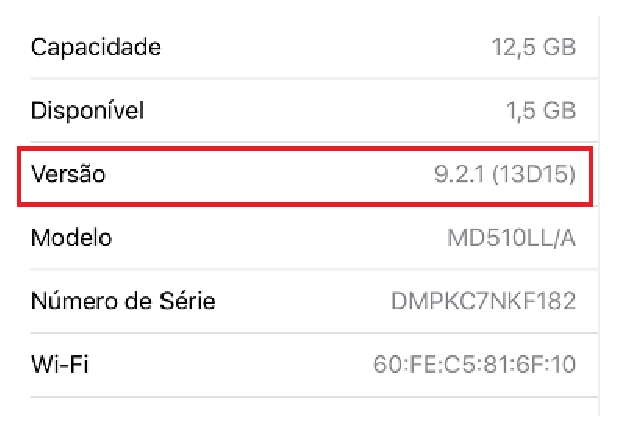
\includegraphics{imagem2.eps}
  \caption{A vers\~ao presente no dispositivo usado para testes, destacada em vermelho}
\end{figure}

Vale lembrar que o autor n\~ao se responsabiliza por eventuais danos causados em dispositivos iOS decorrentes da aplica\c c\~ao das configura\c c\~oes recomendadas aqui. Por isso, \'e sugerido que, se poss\'ivel, estas recomenda\c c\~oes sejam aplicadas inicialmente em aparelhos de teste para, apenas depois, serem aplicadas em outros dispositivos. 

Realizar backups das informa\c c\~oes contidas no dispositivo tamb\'em \'e uma pr\'atica recomend\'avel para a recupera\c c\~ao de informa\c c\~oes importantes, caso ocorram eventuais problemas. Seguem logo abaixo instru\c c\~oes para a realiza\c c\~ao de backups em dispositivos iOS:

\begin{enumerate}
\item Pressionar o \'icone Ajustes
\item Pressionar iCloud
\item Selecionar para backup todas as informa\c c\~oes que o usu\'ario considerar importantes (E-mail, Contatos, etc.)
\item Pressionar Backup
\item Na tela seguinte, ativar Backup do iCloud deslizando o controle para a direita
\item Na mesma tela, caso o usu\'ario esteja conectado a uma rede Wi-Fi, pressionar Efetuar Backup Agora   
\end{enumerate}
